\documentclass{article}
\usepackage{graphicx}
\usepackage[margin=1.5cm]{geometry}
\usepackage{amsmath}

\begin{document}
\twocolumn

\title{Homework 3, Unit 0: Foundations and Fundamentals}
\author{Prof. Jordan C. Hanson}

\maketitle

\section{Memory Bank}
\small
\begin{itemize}
\item \textbf{Homogeneous system:} Let $k$ be a constant, and let $s_{\rm in}(t)$ and $s_{\rm out}(t)$ be the input and output signals to a system $S$, respectively.  $S$ is \textit{homogeneous} if:
\begin{align}
s_{\rm out}(t) &= S[s_{\rm in}(t)] \\
k s_{\rm out}(t) &= S[k s_{\rm in}(t)]
\end{align}
\item \textbf{Additive system:} Let $s_{\rm 1}(t)$ and $s_{\rm 2}(t)$ be two input signals to a system $S$, with outputs $s'_{\rm 1}(t)$ and $s'_{\rm 2}(t)$.  $S$ is \textit{additive} if:
\begin{align}
s'_{\rm 1}(t) &= S[s_{\rm 1}(t)] \\
s'_{\rm 2}(t) &= S[s_{\rm 2}(t)] \\
s'_{\rm 1}(t)+s'_{\rm 2}(t) &= S[s_{\rm 1}(t)+s_{\rm 2}(t)]
\end{align}
\item \textbf{Shift-invariant system:} Let $s_{\rm in}(t)$ and $s_{\rm out}(t)$ be input and output signals to a system $S$, and let $t_0$ be a constant.  $S$ is \textit{shift invariant} if:
\begin{align}
s_{\rm out}(t) &= S[s_{\rm in}(t)] \\
s_{\rm out}(t-t_0) &= S[s_{\rm in}(t-t_0)]
\end{align}
\item $F(f) = \mathcal{F}\left\lbrace f(t)\right\rbrace =\int_{-\infty}^{\infty} f(t) e^{-2\pi jft} dt$ ... The Fourier Transform.
\item $\mathcal{F}^{-1}\left\lbrace F(f)\right\rbrace =\int_{-\infty}^{\infty} F(f) e^{2\pi jft} df$ ... The Inverse Fourier Transform.
\item The \textbf{Dirac $\delta$-function} is a distribution defined by the following property:
\begin{equation}
f(t_0) = \int_{-\infty}^{\infty} f(t) \delta(t-t_0) dt \label{eq:delta}
\end{equation}
In words, the integral of a $\delta$-function times a function $f$ is the value of the function at $t_0$.
\item \textbf{Convolution}: this is an operation that characterizes the response $h[n]$ of a linear system.
\begin{equation}
y[i] = h[n] * x[n] = \sum_{j=0}^{M-1}h[j]x[i-j] \label{eq:conv}
\end{equation}
In words, the output at sample $i$ is equal to the produce of the system response $h$ and the input signal $x$, summed over the proceeding $M$ samples (from $j=0$ to $j=M-1$).
\end{itemize} \vspace{3cm}
\normalsize

\section{Linear Systems}

\begin{figure}[ht]
\centering
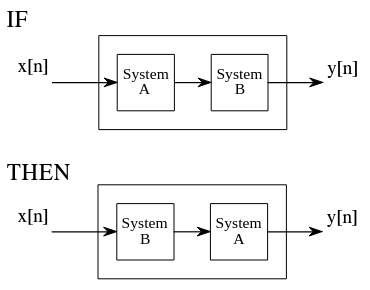
\includegraphics[width=0.25\textwidth]{commute.png}
\caption{\label{fig:1} Linear systems \textbf{commute}.}
\end{figure}

\begin{enumerate}
\item Consider Fig. \ref{fig:1}, which depicts two linear systems A and B.  Symbolically, systems A and B \textbf{commute} if $A\lbrace B\lbrace x[n] \rbrace\rbrace = B\lbrace A\lbrace x[n] \rbrace\rbrace$.  (a) Let $A\lbrace x[n] \rbrace = 2x[n]-1$, and $B\lbrace x[n] \rbrace = 0.5x[n]$.  Which system, A or B, is a linear system?  For the system that is not linear, which linear property does it break? (b) Modify the non-linear system to make it linear, and show that A and B commute. \\ \vspace{4cm}
\item Consider Eq. \ref{eq:delta} in the Memory Bank.  Let $f(t) = a_1\cos(2\pi f_1 t) + a_2\cos(2\pi f_2 t)$, with $T_1 = 1/f_1$, $T_2 = 1/f_2$, and $f_2 = 2f_1$.  Evaluate the following:
\begin{itemize}
\item $\int_{-\infty}^{\infty} f(t) \delta(t-T_1) dt$
\item $\int_{-\infty}^{\infty} f(t) \delta(t-T_2) dt$
\end{itemize} \vspace{4cm}
\item Let $f(t) = a\delta(t-t_0)$.  (a) Show that the magnitude of the \textbf{Fourier transform} of this impulse is $a$. (b) Show that the phase angle, $\phi$, is $-2\pi ft_0$. (c) Show that the group delay, $\tau_g = -d\phi/d\omega$ is $t_0$. \\ \vspace{4cm}
\item Let $\delta[n]$ represent a digital impulse: [1000 0000]\footnote{Let the index for data in this list of numbers start with $n=0$.}. (a) If $y[n] = S[x[n]] = 0.5x[n-2]$, what is $S[\delta[n]]$? (b) $y[n]$ is the \textit{impulse response} of $S$.  What is the \textit{step response}, if the step input is $s[n] = [0111 1111]$? \\ \vspace{4cm}
\end{enumerate}

\section{Fourier Transforms and \\ Basic Filters}

\begin{enumerate}
\item Suppose we pass a signal $s(t)$ into a low-pass filter.  The signal as a function of frequency is $S(f)$, the Fourier transform of $s(t)$.  The output of the low-pass filter will be $S(f)$ times $1/(1+j\omega \tau)$, where $\omega = 2\pi f$, and $\tau = RC$.  That is, the output will be $S(f)/(1+j\omega \tau)$.  (a) Calculate the Fourier transform $S(f)$, if $s(t) = a\delta(t-t_0)$ (as we did in class).  (b) Suppose we pass our impulse $s(t)$ into a low-pass filter.  What is the magnitude of the output, as a function of frequency? (c) Repeat this exercise, but with a high-pass filter response: $j\omega\tau/(1+j\omega \tau)$. \\ \vspace{4cm}
\item For the output spectra of the previous exercise, low-pass and high-pass, calculate the group delays.\footnote{Hint: multiply the numerator and denominator of ratios by the complex conjugate of the denominator, to aid in splitting the complex expression into real and imaginary parts.} \\ \vspace{4cm}
\item (a) Show that the inverse Fourier transform of $S(f) = (a/2)(\delta(f-f_0) + \delta(f+f_0))$ is a cosine function. (b) Show that the inverse Fourier transform of $S(f) = (a/2j)(\delta(f-f_0) - \delta(f+f_0))$ is a sine function. \ \vspace{4cm}
\end{enumerate}

\section{Convolution and Octave Code}

\begin{enumerate}
\item For the following exercises, use Eq. \ref{eq:conv}. Let the digital impulse be $\delta[n]$ which is 1 for $n=0$, and 0 if $n\neq 0$.  For example, $\delta[n-5]$ is 1 when $n=5$. (a) Show that if $x[n] = \delta[n]$, $y[n] = h[n] * x[n] = h[n]$.  That is, if the input data is an impulse, the output is the system response. (b) Show that if the input impulse is shifted ($x[n] = \delta[n-n_0]$), the output is $h[n]$, shifted by the same amount. \\ \vspace{4cm}
\item In \verb+octave+, use the \verb+conv+ function to convolve a 440 Hz sine wave with a $\delta[n-n_0]$ impulse.  Shift the phase of the sine output by varying $n_0$.
\end{enumerate}

\end{document}
